% Title Hrader
\title{\LaTeX Template}
\author{
        Kia Rahmani \\
                Department of Computer Science\\
        Purdue University, USA
}
\date{\today}

% Main Document
\documentclass[12pt]{article}
\usepackage{xcolor,listings}
\usepackage{graphicx}
\usepackage[inline]{enumitem}
\usepackage[utf8]{inputenc}
\usepackage[spanish]{babel}
\usepackage{csquotes}


\begin{document}
%\maketitle
%\begin{abstract} \end{abstract}


% Sections
\section{Low Level Query Translation}
In this document, we will present different SQL queries and
their equivalent in L2 which would constitute the low level part of our naive
NoSQL compiler. 
The low-level part of the compiler focuses on transforming single queries into L2 (in this case
Riak and Antidote) facilities, which are usually executed within a sharded datacenter 
(as oppesed to system-wide distributed transactions)
Translating the input SQL programs (that wrap low-level queries of this
document) will be presented in the next writeup.
\\In the following examples we will assume an input SQL data model:\\
\begin{center}
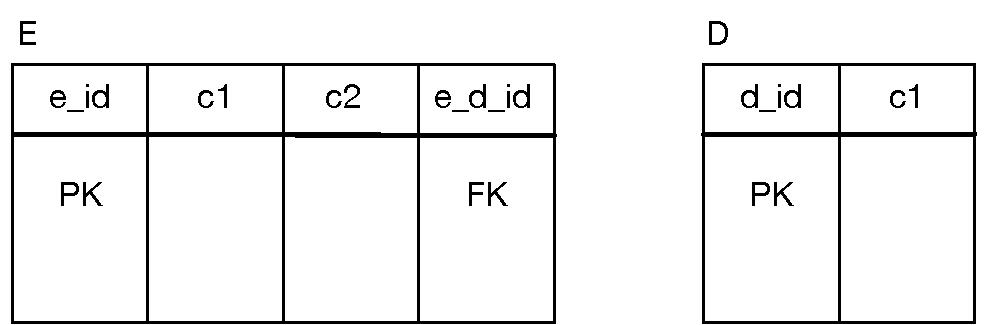
\includegraphics[scale=0.55]{sql_base.pdf}
\end{center}
We also assume that the output of the queries is always
stored in the variable $v$. We also assume full isolation in cases when a node
performs
multiple L2 operations (i.e. there is no interference between operations
of different processes within a single node).
\\We start the translation by presenting the initial L2 objects (we will incrementally update this model
given new queries to be translated):\\ \\
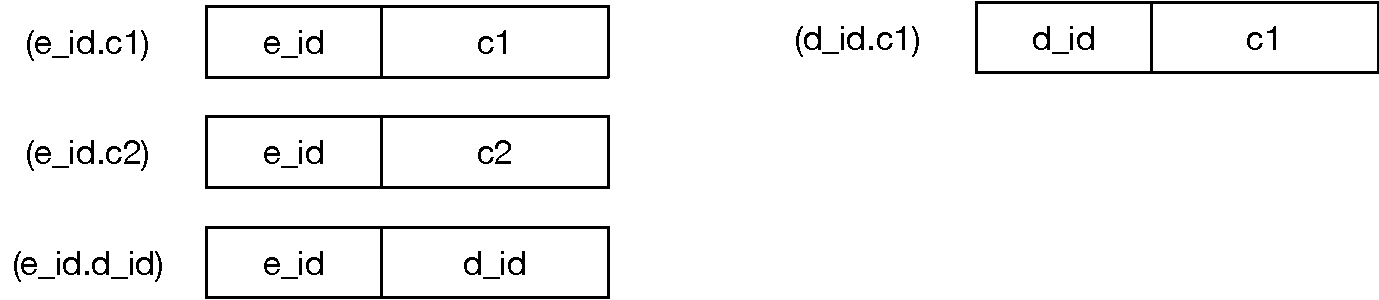
\includegraphics[scale=0.55]{l2_base.pdf}


\subsection{single predicate, equality search}
\begin{enumerate}
\item {On the primary key:}
	\subitem {\bf SQL: } \hspace{5mm}\lstinline[basicstyle=\ttfamily ] 
		{v = SELECT c1 FROM E WHERE (e_id = key)}
	\subitem {\bf L2: } \hspace{7.9mm}\lstinline[basicstyle=\ttfamily ]                        
                {v = (e_id_c1).kvREAD(e_id=key)}
	\subitem
	\subitem {\bf SQL: } \hspace{5mm}\lstinline[basicstyle=\ttfamily ] 
		{v = SELECT * FROM E WHERE (e_id = key)}
	\subitem {\bf L2: } \hspace{7.9mm}\lstinline[basicstyle=\ttfamily ]                        
                {v.fst = (e_id.c1).kvREAD(e_id=key);}
	\subitem \hspace{18.6mm}\lstinline[basicstyle=\ttfamily ]                        
                {v.snd = (e_id.c2).kvREAD(e_id=key);}
	\subitem \hspace{18.6mm}\lstinline[basicstyle=\ttfamily ]                        
                {v.thd = (e_id.d_id).kvREAD(e_id=key)}
\item {On a non-primary key (e.g. c2):}
In this case we have two options:
\begin{enumerate*}
  \item Using a denormalized datamodel which avoids datacenter-wide
	  scans but adds extra anomalies due to the unsync copies of entries.
  \item Using Riak's map-reduce capabilities or Secondary Indexes, both
	  of which
	  are easier to implement and maintain but require data-center
	  wide scans with growing complixty proportional to the number of
	  partitions and the number of entries. Neither of them are recommended for
	  production usage.
\end{enumerate*}
\paragraph{(a) Denormalization:}
We should update the L2 data-model by \emph{adding} two new
buckets: \emph{c1\_by\_c2} and \emph{d.id\_by\_c2}, each keeping
a map from c2 column type to a map from e\_id to c1 and d.id
respectively:


\begin{center}
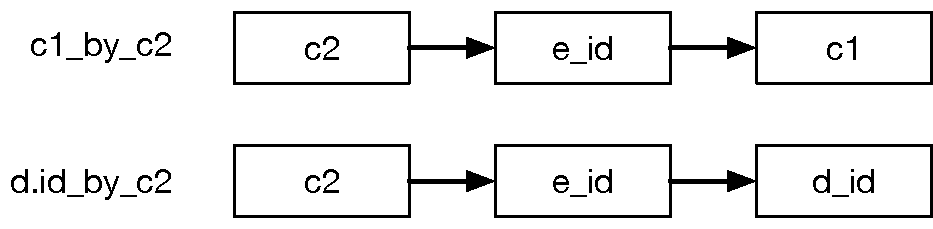
\includegraphics[scale=0.42]{den_obj.pdf}
\end{center}
	\subitem {\bf SQL: } \hspace{5mm}\lstinline[basicstyle=\ttfamily ] 
		{v = SELECT * FROM E WHERE (c2 = key)}
	\subitem {\bf L2: } \hspace{8.5mm}\lstinline[basicstyle=\ttfamily ]                        
                {v1 = (e_id.c1).mapREAD(e_id=key);}
	\subitem \hspace{18.6mm}\lstinline[basicstyle=\ttfamily ]                        
                {v2 = (e_id.d_id).mapREAD(e_id=key)}
	\subitem \hspace{18.6mm}\lstinline[basicstyle=\ttfamily ]                        
		{Let v = zip(v1,v2)}

\paragraph{(b) MapReduce or Secondary Indexing:}
Basho documentations state:
\begin{displayquote}
``We recommend running MapReduce operations in a controlled,
rate-limited fashion and never for realtime querying purposes."
\end{displayquote}
and
\begin{displayquote}
`` If your ring size exceeds 512 partitions, secondary indexes can cause performance
issues in large clusters.''
\end{displayquote}
Which forces us to choose the former approach when designing our compiler.
However, in order to make this document complete we will briefly discuss
them here.
Riak supports simple secondary indexes on objects by tagging them with string or
integer values. The tags indexes are maintained at the same shard where
the data resides (which explains the performance issues when growing the
cluster).
\\ In this example, without denormalizing the data model, we can tag (e\_id.c1) and (e\_id.d\_id) objects
with values of c2 (let's assume c2 is an integer column):

	\subitem {\bf L2: } \hspace{7.9mm}\lstinline[basicstyle=\ttfamily ]                        
	{(keys,v1) = (e_id.c1).get_index('c2', key);}
	\subitem \hspace{18.6mm}\lstinline[basicstyle=\ttfamily ]                        
	{Let v2 = map(k=>(e_id.d_id).kvREAD(e_id=k)) keys }
        \subitem \hspace{18.6mm}\lstinline[basicstyle=\ttfamily ]
	                {Let v = zip(v1,v2)}

As we can see, this approach is not easier than the denormalized
version. We could have made this case a little simpler by changing our
initial fine-grained model into a model where all columns reside in the
same Riak object (coarse grained modeling), which would have eliminated
the need for the iterative reads, but even in that case Riak seems
to update the tag table and the entries in a weakly isolated fashion
which might cause some anomalies\footnote{This claim requires experiments, 
I could not find anything in the documentations}.

\end{enumerate}

\subsection{Multiple predicates, equality search}
Since Riak does not support partial key queries, in this case, we should follow a hybrid approach where we make use of
both denormalization\footnote{Note that, we could have simply used MapReduce
functions without denormalization and allowed DC-wide scans, however the Basho documents state:
"Do NOT use MR when you want to query data over an entire bucket. MapReduce uses a
list of keys, which can place a lot of demand on the cluster."} (if the PK is not used in the predicates) and a
MapReduce function (for filtering out the unwanted entries according to
the rest of the predicates\footnote{Or fetch all entries
satisfying one predicate and trim them locally}). 
\\ For example, if we wanted to query all entries of the table E where 
($\mathtt{c2=key1} \wedge \mathtt{e\_d\_id=key2}$), we could have denormalized the data model and queried riak similar
to
1.1.2.(a) with a map function to filter out the undesired entries: 

\begin{lstlisting}[language=Python,basicstyle=\small,backgroundcolor =
\color{lightgray}]
function(value, keyData, arg){
  var data = Riak.mapValuesJson(value)[0];
  if (data.e_d_id == key2)
    return [ data ]; 
}
\end{lstlisting}

\subsection{Inequality Search (Single/Multiple Predicates)}
\paragraph{} In this case, denormalization does not necessarily eliminate the datacenter-wide scans, 
since the range of keys queried might reside on multiple 
(or even all of the) shards. Note that using MapReduce functions we can collect the entries satisfying all predicates from the shards in the DC, however, there is no guarantee that the entries 
from different shards would be from the same version. 
\\ For example, 
consider a datacenter with three shards. After S1 queries S2 and S3 to collect 
a set of entries, and after S2 computes its response, a new remote range update might arrive at the datacenter. 
Now S3's result is going to contain the newly arrived update but S2's result
lacks it. This anomaly which would cause an inconsistent state read on range
queries, does not exist in unsharded databases (and trivially in relational databases). 
\paragraph{} Riak and other well known NoSQL stores do not provide any
facitility that could be used to fix this problem (I guess since the connections within a DC are usually very fast, 
this problem is not prevalent in production. However since we are bulding a
verified implementation we should handle and eliminate this anomaly as well).
\\ In order to avoid this anomaly, we can use higher level facilities usually
offered by extension
tools running on kv-stores. For example we can use Antidote's read-only (write-only) transactions
to guarantee that all such queries (range updates) end up accessing
(updating) the database instantaneously. \\
In the following example, I will sketch the translation of a simple range query.
The high-level program translation which I will present in the next write-up
will include exact notions of WO and RO transactions of Antidote and our general
purpose compilation scheme.


\paragraph{Example:} Assume a simple case where we want to query c1 field of all the entries from E
with ids less than 100:




\begin{itemize}
\item {\bf SQL: } \hspace{5mm}\lstinline[basicstyle=\ttfamily]{v = SELECT c2 FROM E WHERE (c1 < 100)}
\\ 
\begin{center}
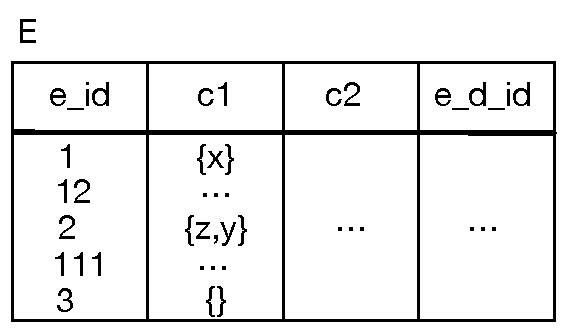
\includegraphics[scale=0.55]{range_ex.pdf}
\end{center}

\item {\bf L2}:
\begin{lstlisting}[language=C,basicstyle=\small,backgroundcolor =
\color{lightgray}]
\\ first create a list of object/keys to be read
for i in [0..100]:
	Obj[i] = {i, antidote_crdt_set,e_id_c1}

\\ read values from the given key-list in a transaction
{ok, Result, CT2} = 
	rpc:call(Node, antidote, read_objects,
	[CT1, [],Obj]).

\\Result[1]= {x}
\\Result[2]= {z,y}
\\Result[3]= {}
\\ ...
\end{lstlisting}

\end{itemize}






















% The Biblography
%\bibliographystyle{abbrv}
%\bibliography{../kia-bib}
\end{document}
